\begin{figure}[H] \centering
\subsection{BDD (SK)}
{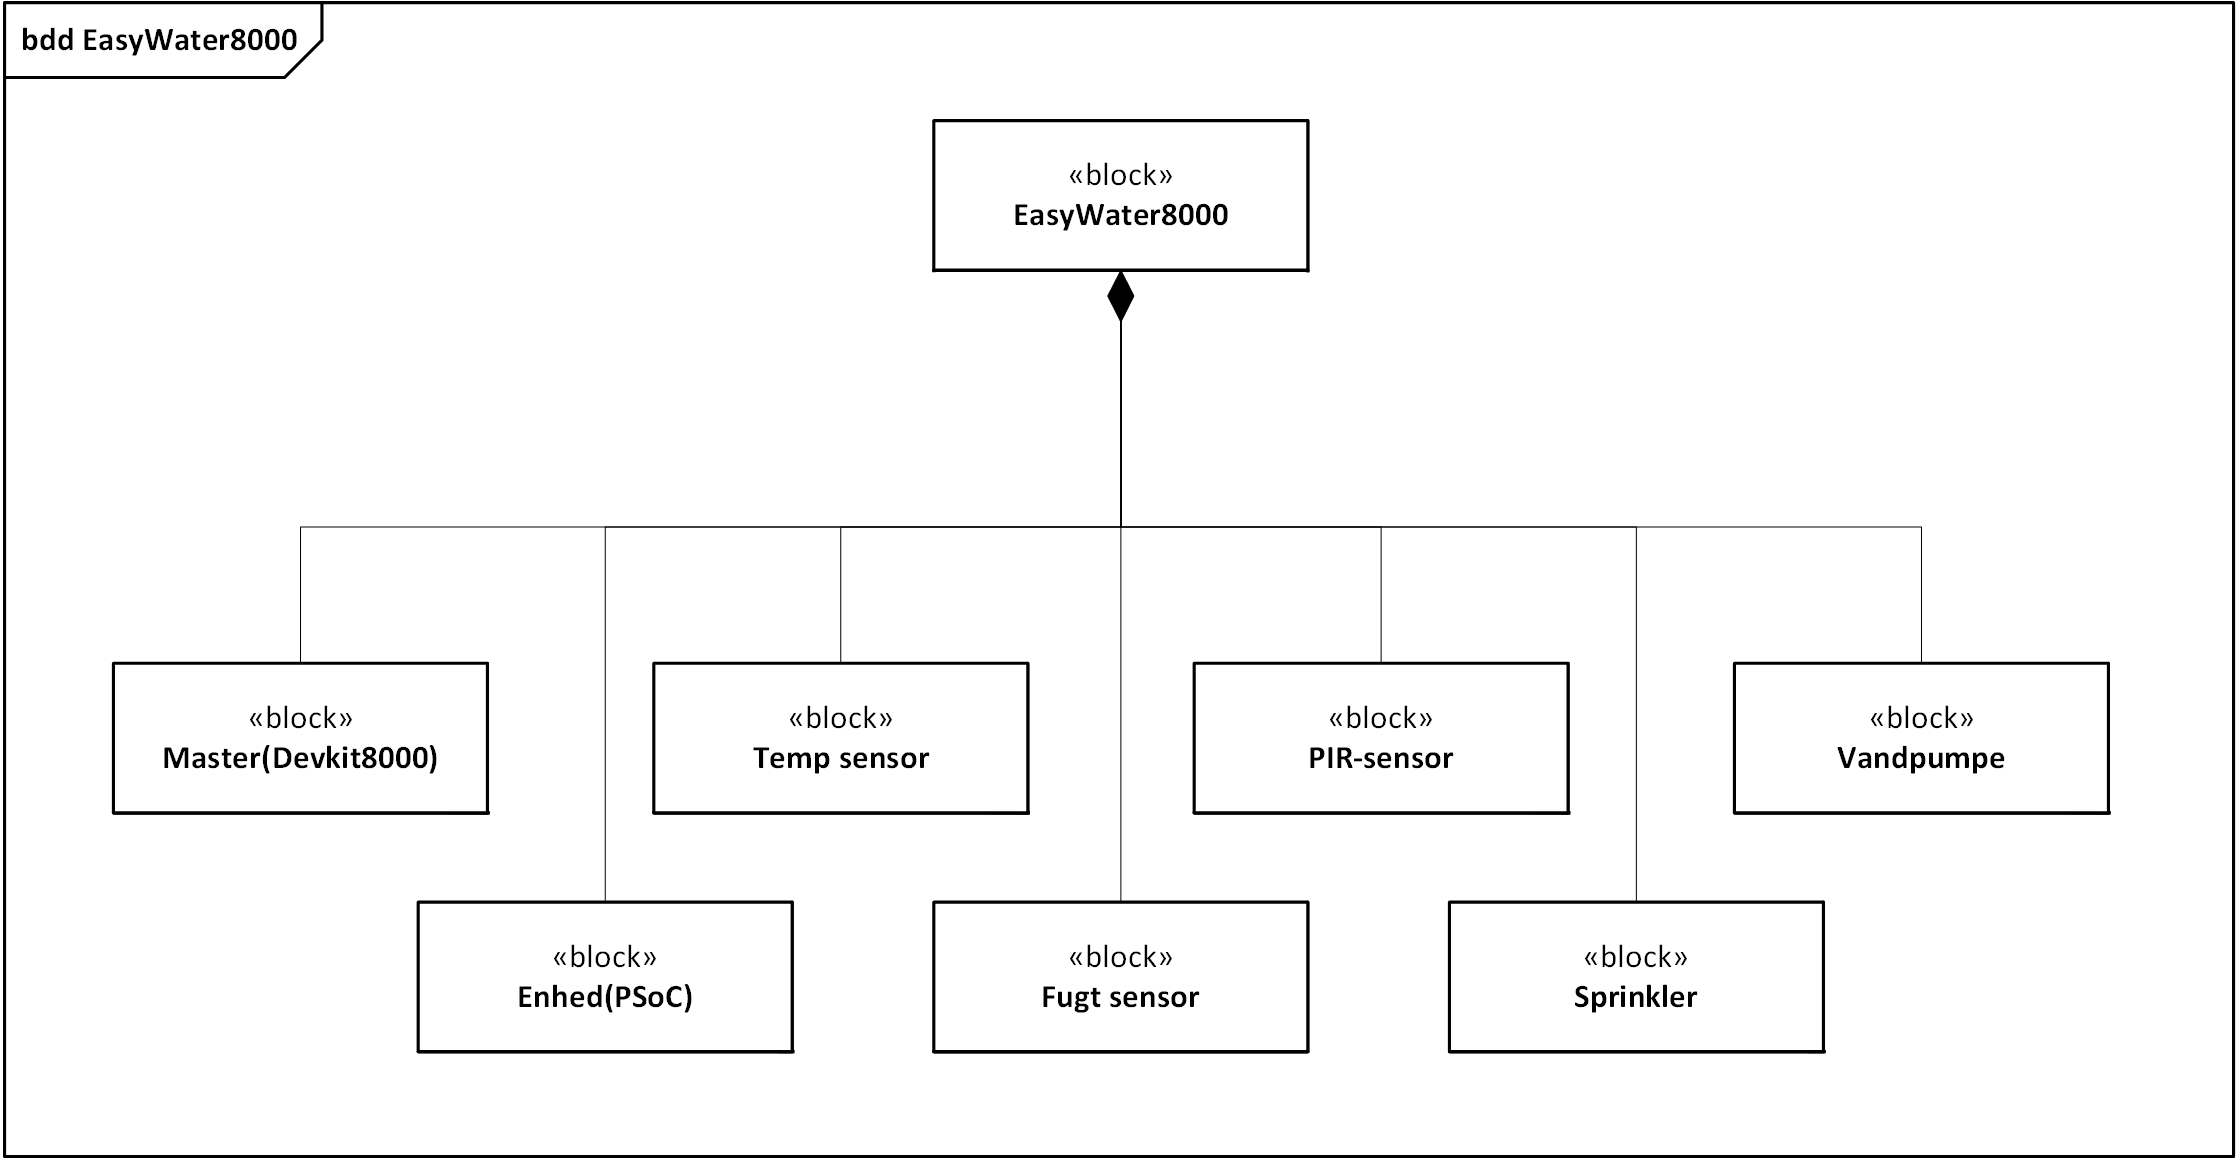
\includegraphics[width=0.9\textwidth]{filer/systemarkitektur/BDD}}
\caption{BDD}
\label{lab:bdd}
\raggedright
\end{figure}
BDD diagrammet giver et overblik over hvad det samlede system består af. \newline \newline
\textbf{Master(Devkit8000)}: Devkit8000 er Master der styrer hele systemet, den modtager inputs fra en touchskærm.  \newline \newline
\textbf{Enhed(PSoC)}: PSoC'en er grænsefladen til den fysiske verden, den indsamler data fra sensorer. Den modtager ordre fra Devkit8000 der styrer hvad der skal ske. 		\newline \newline
\textbf{Temperatursensor}: Har til opgave at indsamle temperaturmålinger. \newline \newline
\textbf{Fugtsensor}: Har til opgave at indsamle fugtighedsmålinger. \newline \newline
\textbf{PIR-sensor}: Har til opgave at detektere om der er bevægelse på banen. \newline \newline
\textbf{Sprinkler}: Har til opgave at sprede vand ud på banen. \newline \newline
\textbf{Vandpumpe}: Har til opgave at forsyne sprinkleren med vand. \newline \newline

\begin{figure}[H] \centering
\subsection{BDD Master (MK)}
{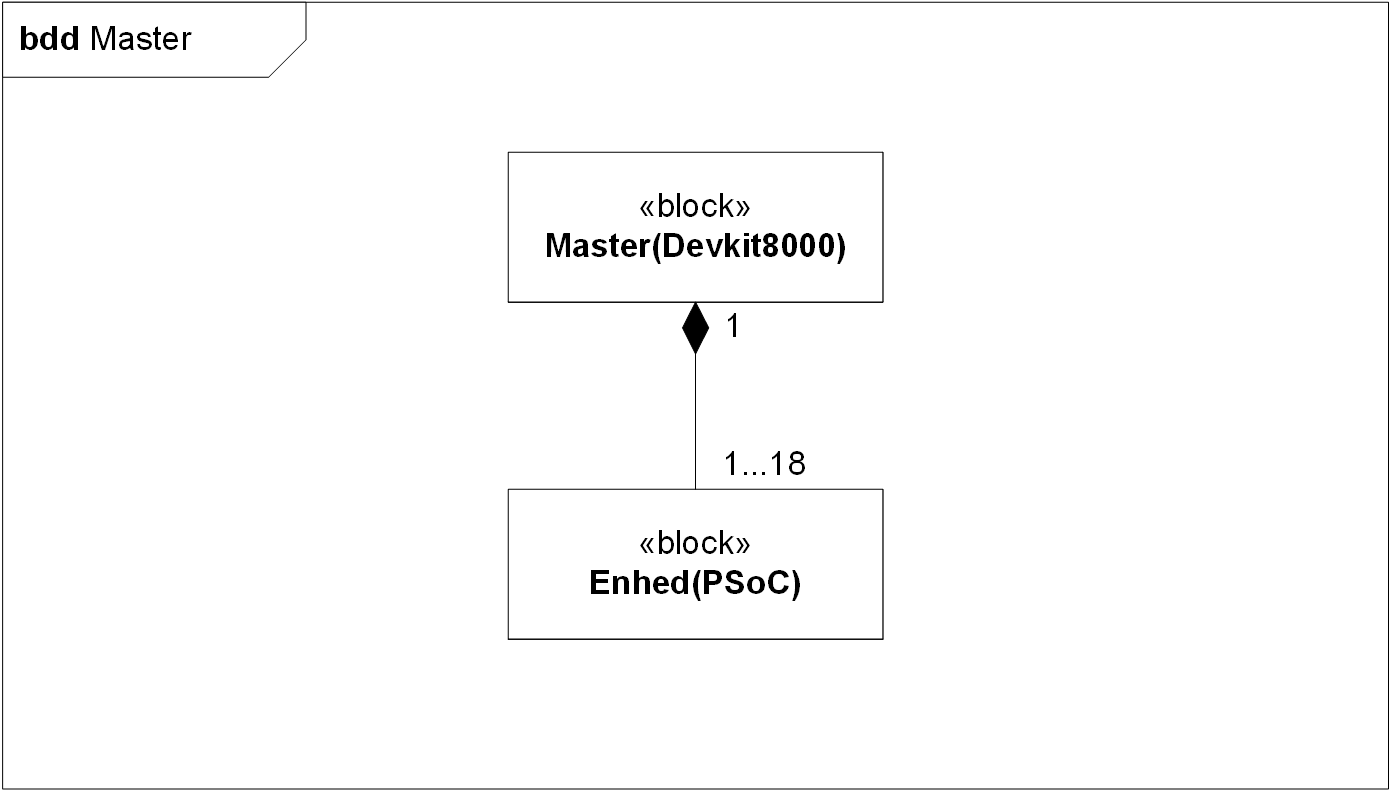
\includegraphics[width=0.9\textwidth]{filer/systemarkitektur/BDD_Master}}
\caption{BDD Master}
\label{lab:bddmaster}
\raggedright
\end{figure}
BDD diagrammet for Master, viser at Master består af et Devkit8000, som kobles op med op til 18 Enheder.

\begin{figure}[H] \centering
\subsection{BDD Enhed (MK)}
{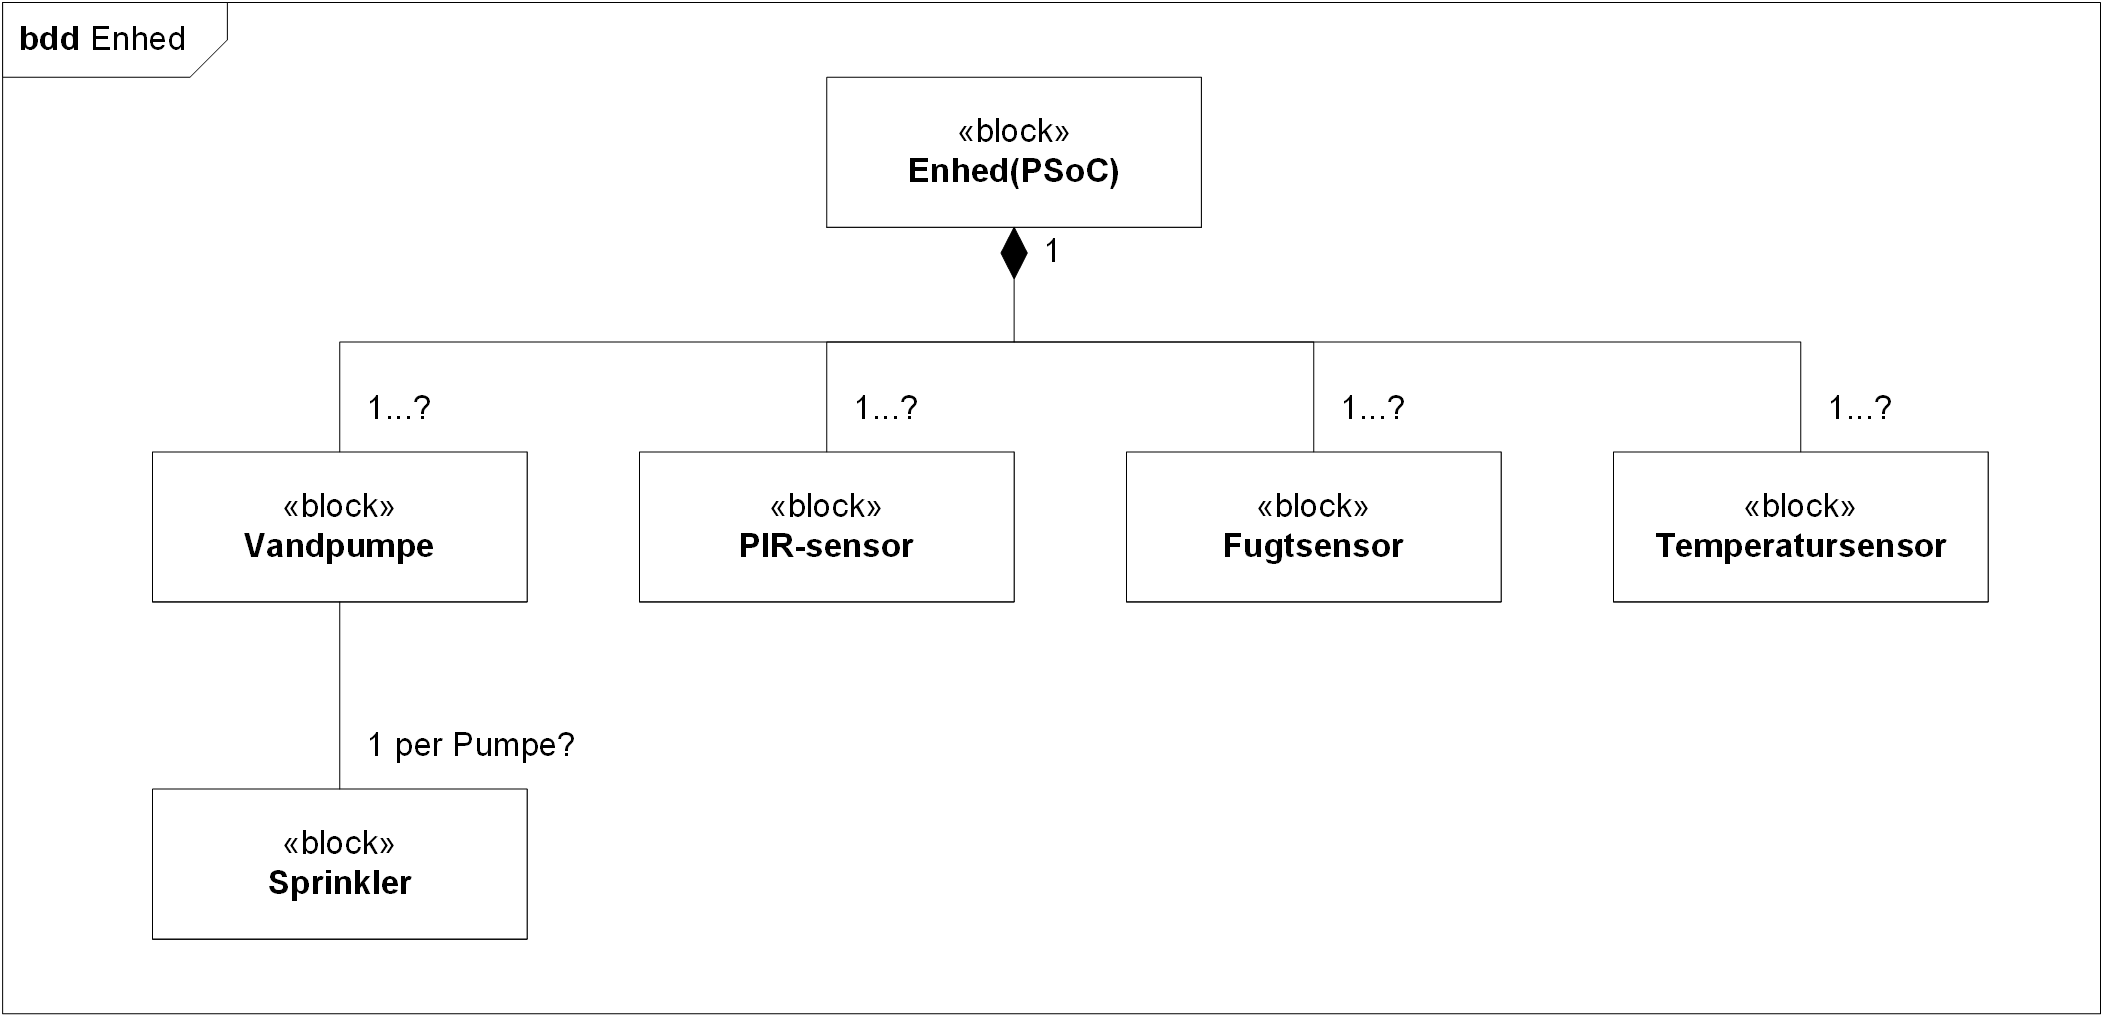
\includegraphics[width=0.9\textwidth]{filer/systemarkitektur/BDD_Enhed}}
\caption{BDD Enhed}
\label{lab:bddenhed}
\raggedright
\end{figure}
BDD diagrammet for Enhed, viser at én Enhed består af én PSoC som kan kobles sammen med op til 20 Vandpumper, 20 Fugtsensorer og 20 Temperatursensorer samt 1 PIR-sensor. Sprinkler bliver i systemet koblet sammen med én Vandpumpe.

\begin{figure}[H] \centering
\subsection{IBD (SK)}
{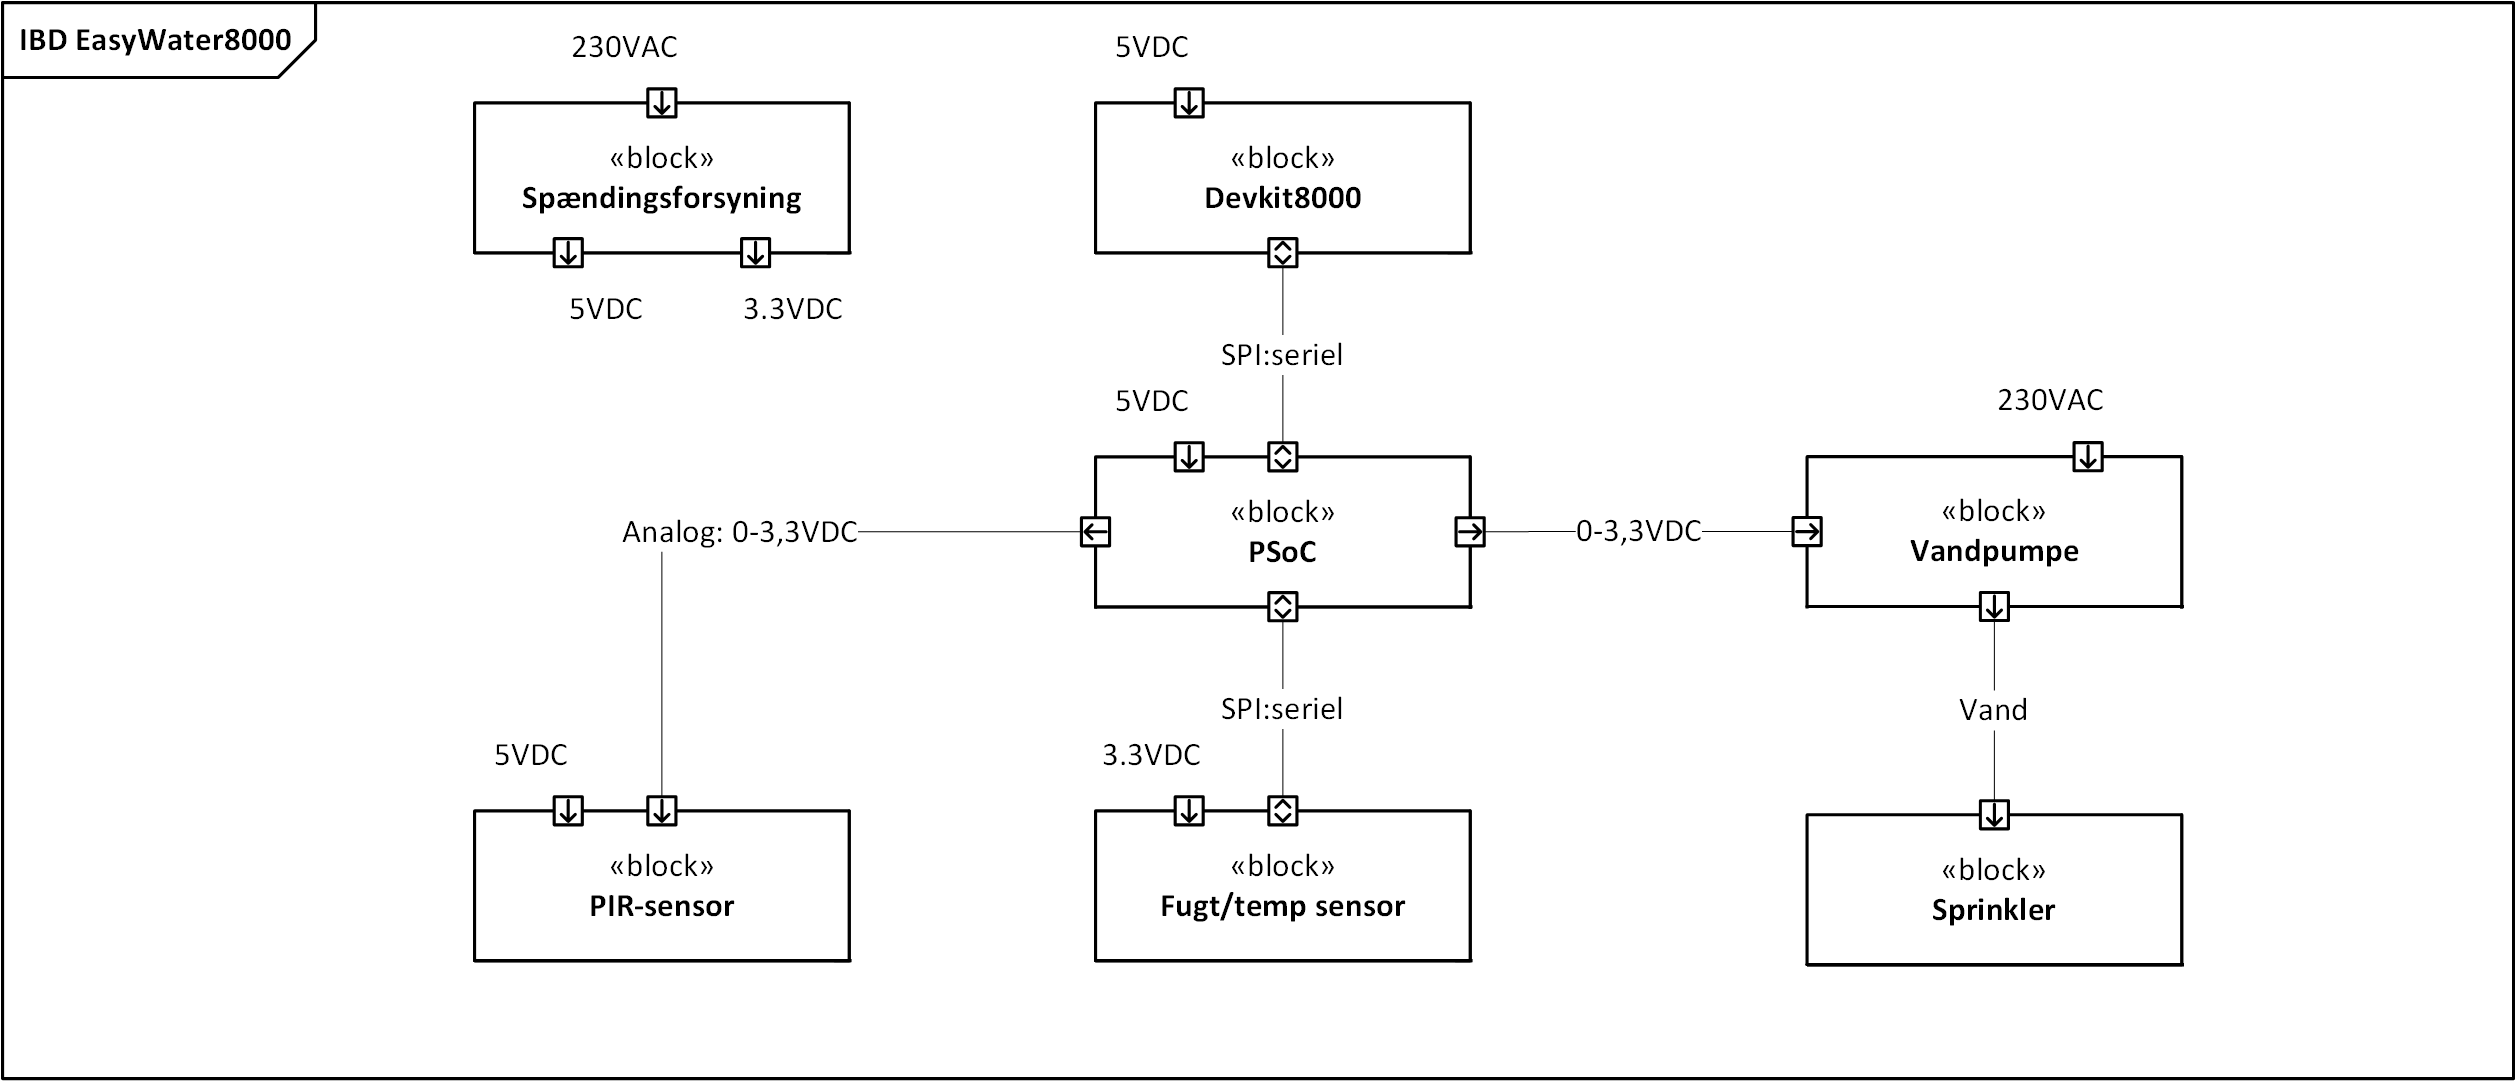
\includegraphics[width=0.9\textwidth]{filer/systemarkitektur/IBD}}
\caption{IBD}
\label{lab:ibd}
\raggedright
\end{figure}
IBD diagrammet giver et internt overblik over hvordan hele vores system er forbundet. Vi ser hvilke type signaler der bliver sendt imellem de forskellige blokke. \newline \newline
\textbf{Spændingsforsyning}: Spændingsforsyningens forbindelser er ikke påtegnet da dette ville give et uoverskueligt diagram, de er i stedet beskrevet med standardflowports.  \newline \newline
\textbf{Integreret fugt- og temperatursensor}: Blokken beskriver at fugt- og temperatursensor er integreret i en chip. \newline \newline

\begin{table}[H]
\subsection{Signal beskrivelse (HW)}
For at fuldende beskrivelsen af grænsefladen er der lavet en signaltabel som kan ses herunder. Hvert signal er beskrevet og tilknyttet en kort kommentar. Området et signal er defineret under, er også beskrevet. Blok og terminal indgår også. 
\caption{Tabel over signaler med terminaler}
\begin{small}
\begin{tabular}{|p{2cm}|p{2cm}|p{2cm}|p{2cm}|p{2cm}|p{2,2cm}|}
\hline

\textbf{Signal-navn}	&\textbf{Funktion} 		&\textbf{Område} &\textbf{Port 1} 	&\textbf{Port 2} 			&\textbf{Kommentar} \\ \hline

SPI 					&Seriel kommunikation 	& 				&Master (DK\_02)		&Enhed (P\_DK)				&					\\\cline{4-5}
					&						&				&Enhed (P\_FT)		&Fugt-/tempsensor (FT\_01)	&					\\ \hline

TTL 					&TTL 					&0\slash3,3V 	&PIR-sensor (PIR\_01) &Enhed (P\_PIR)			&					\\\cline{4-5}
					&						&				&Enhed (P\_VP)		&Vandpumpe (VP\_01)			&					\\ \hline

\end{tabular}
\end{small}
\label{table:Signaltabel}
\end{table}
